% -*- TeX-master: "../dipole_ilya_paper.tex" -*-
\section{Sample Details}

\begin{figure}[h]
  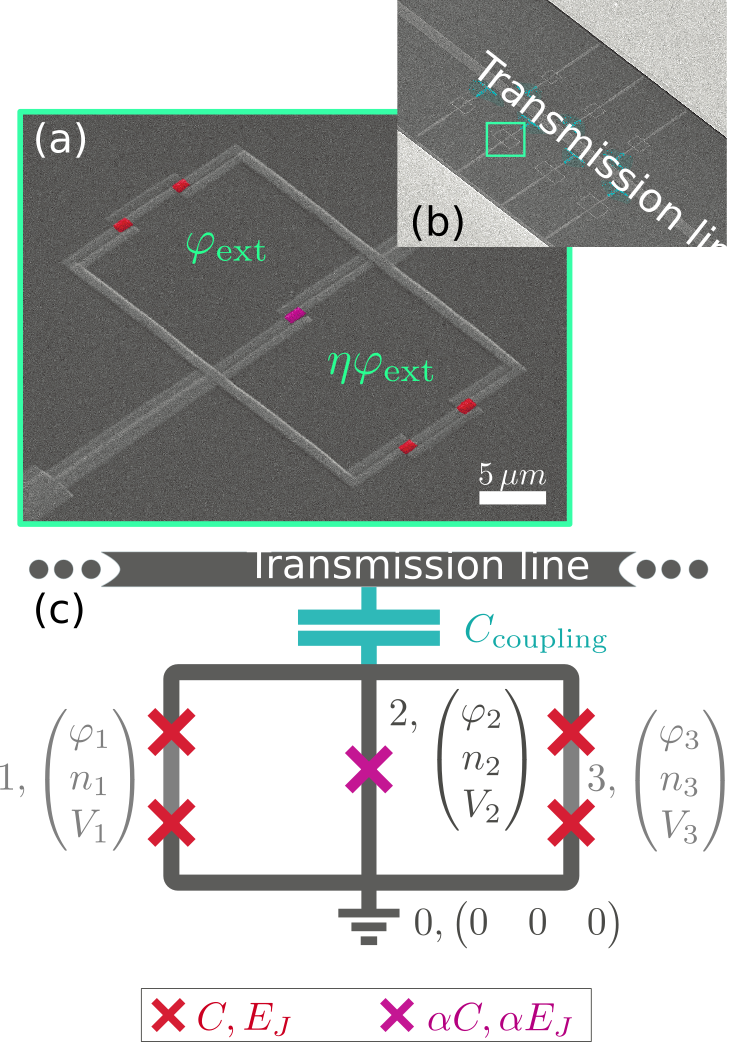
\includegraphics[height=10.5cm]{fig1}
  \caption{\small \textbf{Geometry of a twin qubit:} a) Scanning electron microscope image of
    the twin  qubit. The Al-AlO$_x$-Al JJs  are highlighted in red  and pink; b) Each  of the
    qubits is coupled to  the transmission line with a T-shaped capacitor;  c) The twin qubit
    is  a   symmetrical  arrangement  of  two   individual  flux  qubits  (as   described  in
    \cite{orlando1999})  sharing the  central JJ.   Islands are  labeled with  a Cooper  pair
    occupation n$_i$, phase $\varphi_i$ and voltage V$_i$, with the ground setting a reference of 0
    for all  three variables.   JJs (marked  with crosses)  mediate capacitive  and Josephson
    interactions between  the islands.  The  central junction has  a capacitance of  $\alpha$C and
    Josephson  energy $  \alpha$E$_{J}$, compared  with C$_J$,  E$_J$ of  the outside  ones. Phase
    biases $\varphi, \eta \varphi$,  are applied to the two superconducting loops  with an external magnetic
    field.}
  \label{fig:setup}
\end{figure}

%% Describe fabrication
\noindent  The  qubits  and transmission  line  are  fabricated  on  an undoped  100  silicon
substrate, which is  pre-patterned with 10\,nm NiCr\,-\,90\,nm Au ground  planes. We begin by
cleaning the wafer for  $\sim$~10 minutes at 60\,C in acetone rinsing  in de-ionized water.  Two
layers of electron resist are sequentially spun and post baked (3\,minutes at 60\,C) onto the
wafer:  {Copolymer 13\%},  700\,nm;  ZEP520a:Anisol 2:1,  60\,nm.  We  use  an electron  beam
lithographer  to  expose  the resist  using  a  30\,kV,  10\,pA  beam delivering  a  dose  of
$ 70\,\mu $C/cm$^2$.  The exposed pattern is  developed in P-xylene for 35\,seconds followed by
a 5\,minute  submersion in  IPA:H$_2$0 93:7  and rinse  in pure  IPA.  Shadow  evaporation of
aluminum (Al) in a Plassys simultaneously deposits the JJs and the transmission line.  Plasma
cleaning with  argon before  the deposition of  Al removes residual  resist and  ensures good
galvanic contact  to the gold  pattern. Deposit of  20\,nm of Al  is carried in  situ without
breaking of vacuum followed by static oxidation for 10 minutes at 0.3\,mBar. The intermediate
AlO$_x$ insulating layer is formed at the surface  of Al, which serves as a tunnel barrier of
the JJ.  A second 30\,nm layer of Al completes the process.

These steps give us the 5-JJ structure of the twin qubits. Qubits are capacitively coupled to
the transmission line through T-shaped capacitors,  see Fig.~\ref{fig:setup}.  Each JJ has an
a  area   of  \iunit{400\times200}{nm$^2$}.   The   coplanar  transmission  line   with  impedance
$ Z_{0} \sim 50\,\Omega $ runs to the opening between the ground planes in the center of the chip.

%% Describe setup
We  bond the  sample  chip to  a  printed circuit  board and  mount  it on  a  holder with  a
superconducting-coil   magnet  on   the  13\,mK   stage  of   a  dilution   refrigerator.   A
superconducting shield is used to screen the  holder from stray magnetic fields. The RF lines
connected  to the  sample have  attenuators for  thermalization: -50\,dBm  on the  50K stage,
-30\,dBm on  the 4\,K stage.  We  attach a circulator on  the output line for  isolation. The
transmitted  signal is  amplified  by  +35\,dBm on  the  4K stage  and  by  +35\,dBm at  room
temperature.  This set of attenuators and  amplifiers facilitate power conversion between the
laboratory equipment and qubit microwaves.  Prior to performing characterization measurement,
we  took  the  microwave transmission  spectrum  with  the  qubit  detuned, and  correct  all
measurements by the background transmission profile.

In this  work we  did not  to go  to the  depths of  chemical and  physical treatment  of the
substrate  surface   to  remove  two-level  system   defects  in  the  silicon   oxide  layer
\cite{earnest2018} or employing infra-red filters to eliminate stray light during measurement
\cite{barends2011}, which would improve the parameters of the qubit. Rather we concentrate on
revealing the intrinsic potential of the twin  qubit design and the challenges that will have
to be addressed in the future.

%%% Local Variables:
%%% mode: latex
%%% TeX-master: "../dipole_ilya_paper"
%%% End:
